\section{Monte Carlo Signal Samples}
%\label{section:MCSignalSamples} % uncomment if label used.

\subsection{String signal samples}
%\label{section:MCStringSamples} % uncomment if label used.

The string-resonance samples are generated using the \str version 1.00
Monte Carlo event
generator~\cite{Vakilipourtakalou:2018pfo}.~\footnote{The code can be
obtained from the HEPForge
repository \url{https://strings.hepforge.org/}.} 
The generator outputs LHE files~\cite{Alwall:2006yp} which are upload
to the rucio storage element for ATLAS official Monte Carlo production.
This generator was first made available in ATLAS
release 21.6.7,\texttt{AthGeneration}.   
We use this release and get the following versions for the axillary
programs: \pythia~8.240, Lhapdf~6.2.3~\cite{Buckley:2014ana}, and
EvtGen~1.6.0. 
The generation was validated with
release 21.2.6.0,\texttt{AthDerivation} using \texttt{TRUTH1} n-tuples
prior to official ATLAS Monte Carlo production.

After ATLAS Monte Carlo production of the string samples, errors were
found in the cross section calculations and the relative event
generation of each subprocess.
The event kinematics are correct.
By using the cross sections in Table~\ref{tab1} one recovers the
correct signal strength of each sample for different \Ms.
If one wishes to distinguish the correct contribution of each
subprocess, the events should be weighted according to the values in
Table~\ref{tab3}. 
Using the PDG identifiers of the intial-state partons in the n-tuple
and the corrections in Table~\ref{tab3}, the MC weights branch of the
n-tuple has been filled. 
These weights are to be using in the same way as a MC generator with
weighted events.  

\begin{table}[htb]
\begin{center}
\begin{tabular}{crrrrr}\hline\\[-2ex]
Subprocess             & \multicolumn{5}{c}{\Ms {[TeV]}}\\
& \multicolumn{1}{c}{7.0} & \multicolumn{1}{c}{7.5} &
\multicolumn{1}{c}{8.0} & \multicolumn{1}{c}{8.5} &
\multicolumn{1}{c}{9.0}\\ \\[-2ex]
\hline\\[-2ex]
$gg\to q\bar{q} + gg$  & 2.836 & 2.161 & 2.457 & 2.422 & 1.569\\
$gq\to gq$             & 0.901 & 0.924 & 0.930 & 0.939 & 0.951\\
$g\bar{q}\to g\bar{q}$ & 4.857 & 5.780 & 3.587 & 4.591 & 6.213\\
$q\bar{q}\to gg$       & 1.158 & 1.164 & 1.175 & 1.136 & 1.153\\
\\[-2ex] \hline
\end{tabular}
\end{center}
\caption{Monte Carlo string-resonance subprocess event weights.}
\label{tab3}
\end{table}

The string-resonance samples used in this analysis are shown in
Table~\ref{tab4}. 
Equal sizes of 20000 events were produced for mc16a, mc16d, and mc16e.
The samples were simulated with Atlfast-2.

\begin{sidewaystable}[p]
\begin{small}
\begin{tabular}{l}
\hline
mc16\_13TeV.312404.STRINGSPythia8EvtGen\_A14CTEQ6L1\_STR\_Ms07000.deriv.DAOD\_EXOT2.e7655\_a875\_r9364\_p3929/\\
mc16\_13TeV.312404.STRINGSPythia8EvtGen\_A14CTEQ6L1\_STR\_Ms07000.deriv.DAOD\_EXOT2.e7655\_a875\_r10201\_p3929/\\
mc16\_13TeV.312404.STRINGSPythia8EvtGen\_A14CTEQ6L1\_STR\_Ms07000.deriv.DAOD\_EXOT2.e7655\_a875\_r10724\_p3929/\\
\\
mc16\_13TeV.312405.STRINGSPythia8EvtGen\_A14CTEQ6L1\_STR\_Ms07500.deriv.DAOD\_EXOT2.e7655\_a875\_r9364\_p3929/\\
mc16\_13TeV.312405.STRINGSPythia8EvtGen\_A14CTEQ6L1\_STR\_Ms07500.deriv.DAOD\_EXOT2.e7655\_a875\_r10201\_p3929/\\
mc16\_13TeV.312405.STRINGSPythia8EvtGen\_A14CTEQ6L1\_STR\_Ms07500.deriv.DAOD\_EXOT2.e7655\_a875\_r10724\_p3929/\\
\\
mc16\_13TeV.312406.STRINGSPythia8EvtGen\_A14CTEQ6L1\_STR\_Ms08000.deriv.DAOD\_EXOT2.e7655\_a875\_r9364\_p3929/\\
mc16\_13TeV.312406.STRINGSPythia8EvtGen\_A14CTEQ6L1\_STR\_Ms08000.deriv.DAOD\_EXOT2.e7655\_a875\_r10201\_p3929/\\
mc16\_13TeV.312406.STRINGSPythia8EvtGen\_A14CTEQ6L1\_STR\_Ms08000.deriv.DAOD\_EXOT2.e7655\_a875\_r10724\_p3929/\\
\\
mc16\_13TeV.312407.STRINGSPythia8EvtGen\_A14CTEQ6L1\_STR\_Ms08500.deriv.DAOD\_EXOT2.e7655\_a875\_r9364\_p3929/\\
mc16\_13TeV.312407.STRINGSPythia8EvtGen\_A14CTEQ6L1\_STR\_Ms08500.deriv.DAOD\_EXOT2.e7655\_a875\_r10201\_p3929/\\
mc16\_13TeV.312407.STRINGSPythia8EvtGen\_A14CTEQ6L1\_STR\_Ms08500.deriv.DAOD\_EXOT2.e7655\_a875\_r10724\_p3929/\\
\\
mc16\_13TeV.312408.STRINGSPythia8EvtGen\_A14CTEQ6L1\_STR\_Ms09000.deriv.DAOD\_EXOT2.e7655\_a875\_r9364\_p3929/\\
mc16\_13TeV.312408.STRINGSPythia8EvtGen\_A14CTEQ6L1\_STR\_Ms09000.deriv.DAOD\_EXOT2.e7655\_a875\_r10201\_p3929/\\
mc16\_13TeV.312408.STRINGSPythia8EvtGen\_A14CTEQ6L1\_STR\_Ms09000.deriv.DAOD\_EXOT2.e7655\_a875\_r10724\_p3929/\\
\hline
\end{tabular}
\end{small}
\caption{ATLAS Monte Carlo string-resonance samples.}
\label{tab4}
\end{sidewaystable}

\subsection{String resonance angular distributoon}

\begin{figure}[htb]
\begin{center}
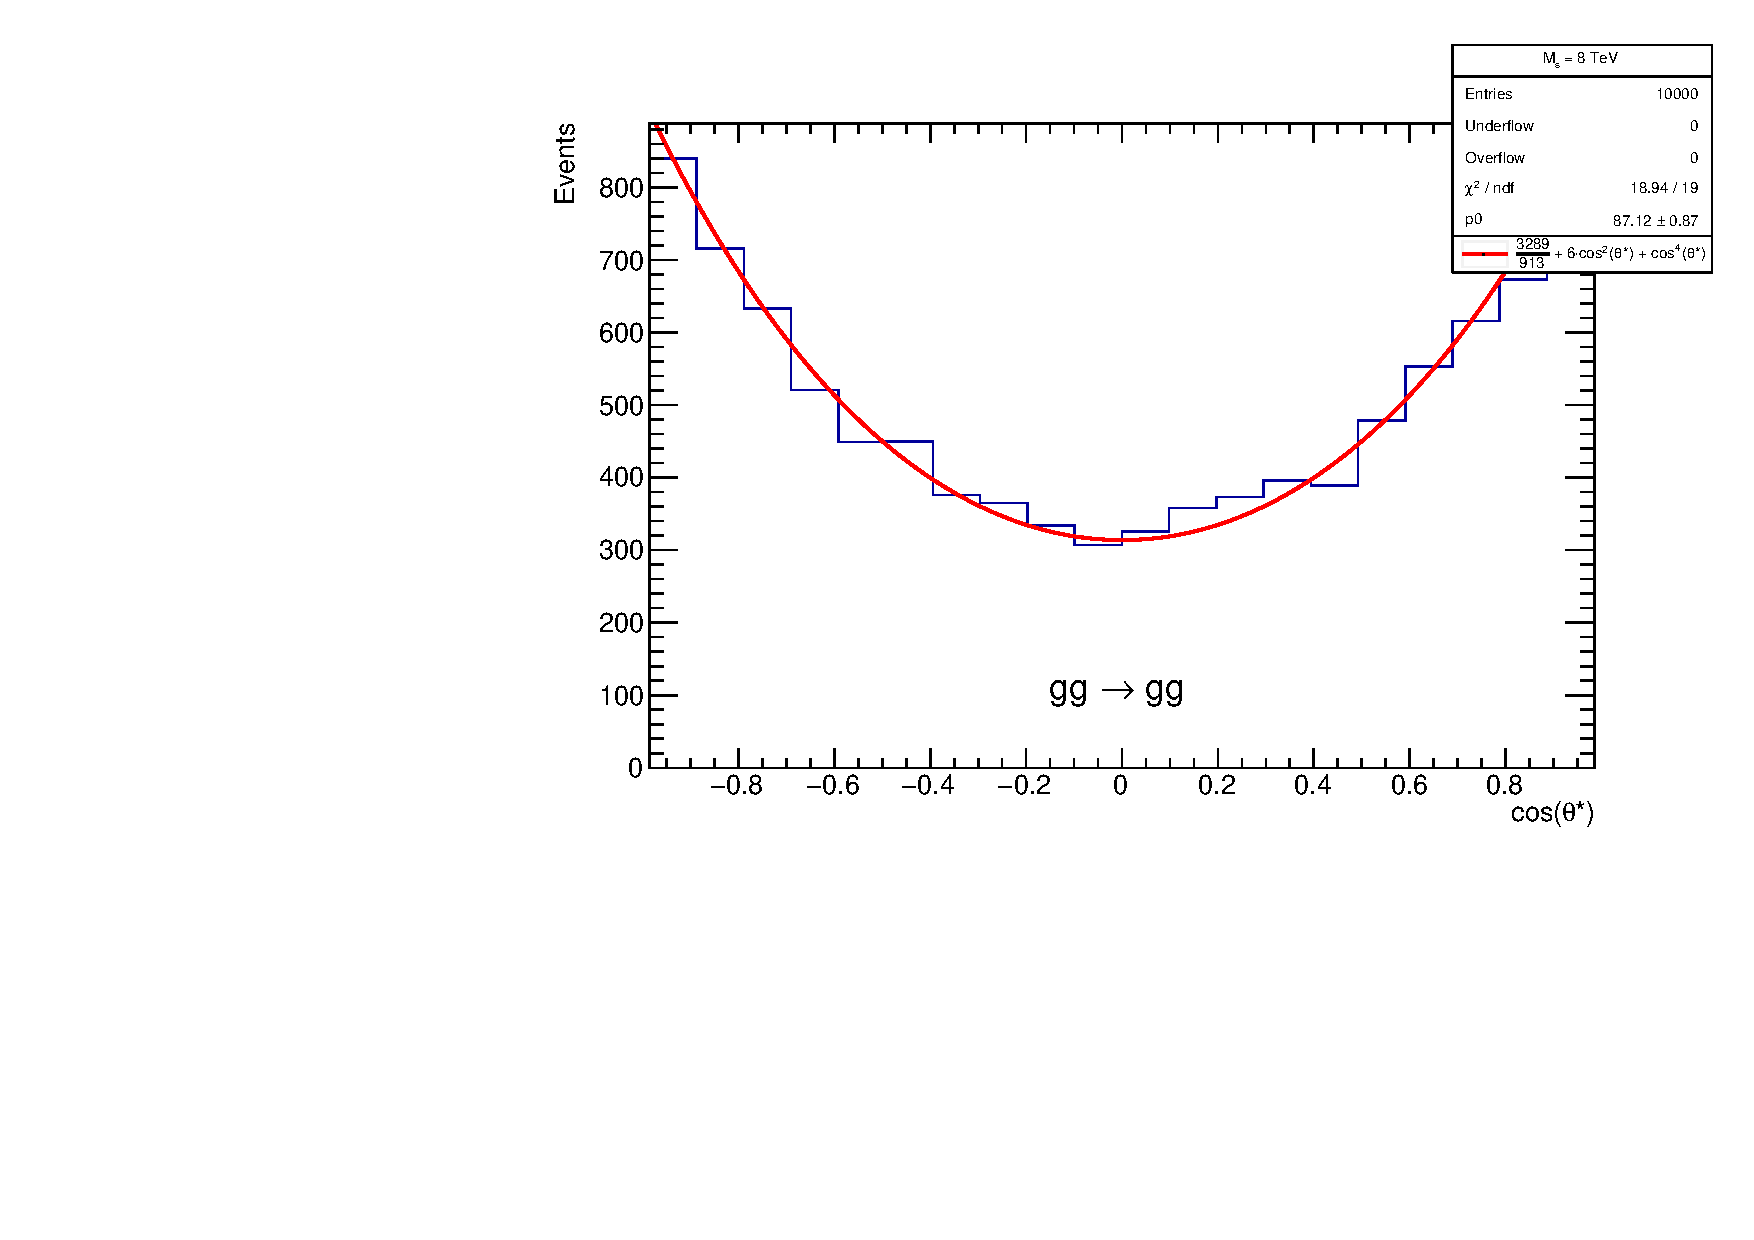
\includegraphics[width=0.45\linewidth]{../figures/strings/angle_gg_gg}
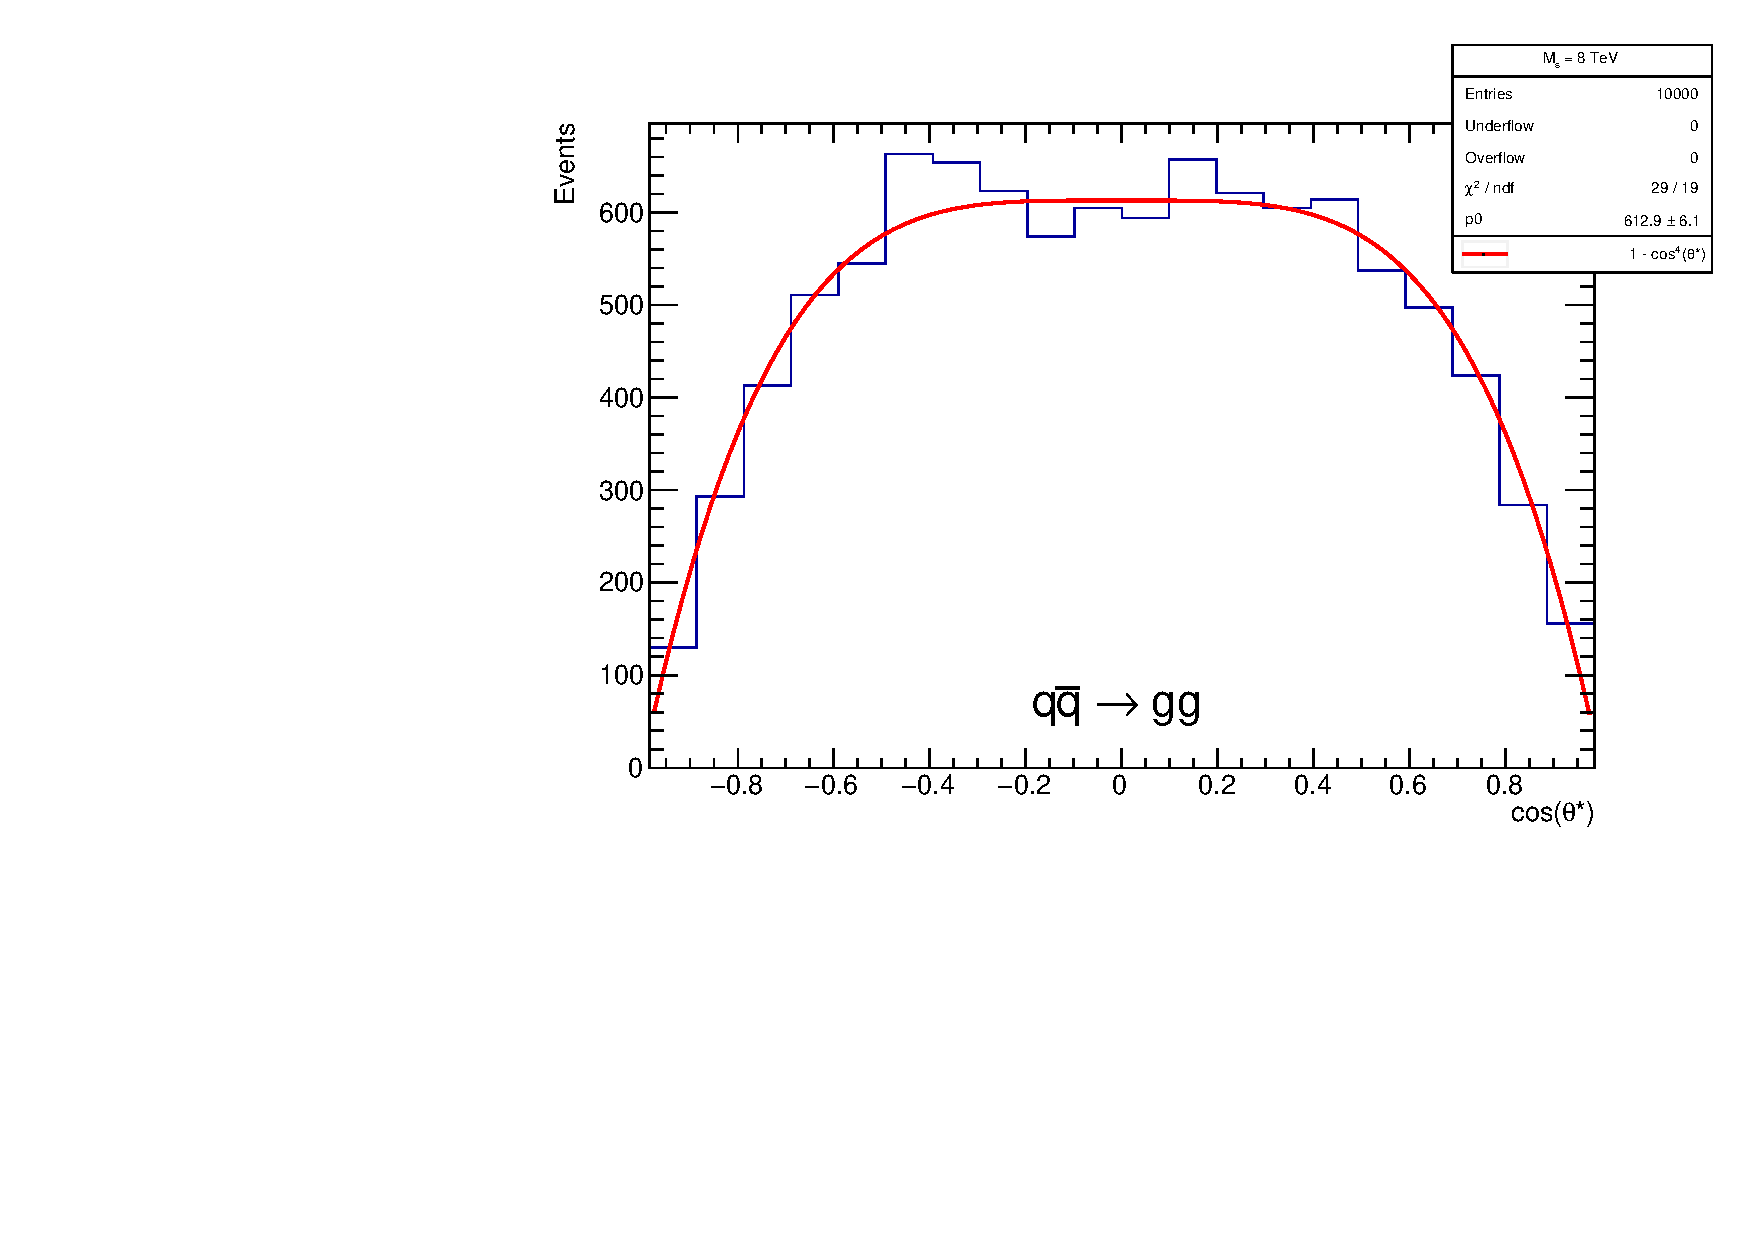
\includegraphics[width=0.45\linewidth]{../figures/strings/angle_qq-bar_gg}
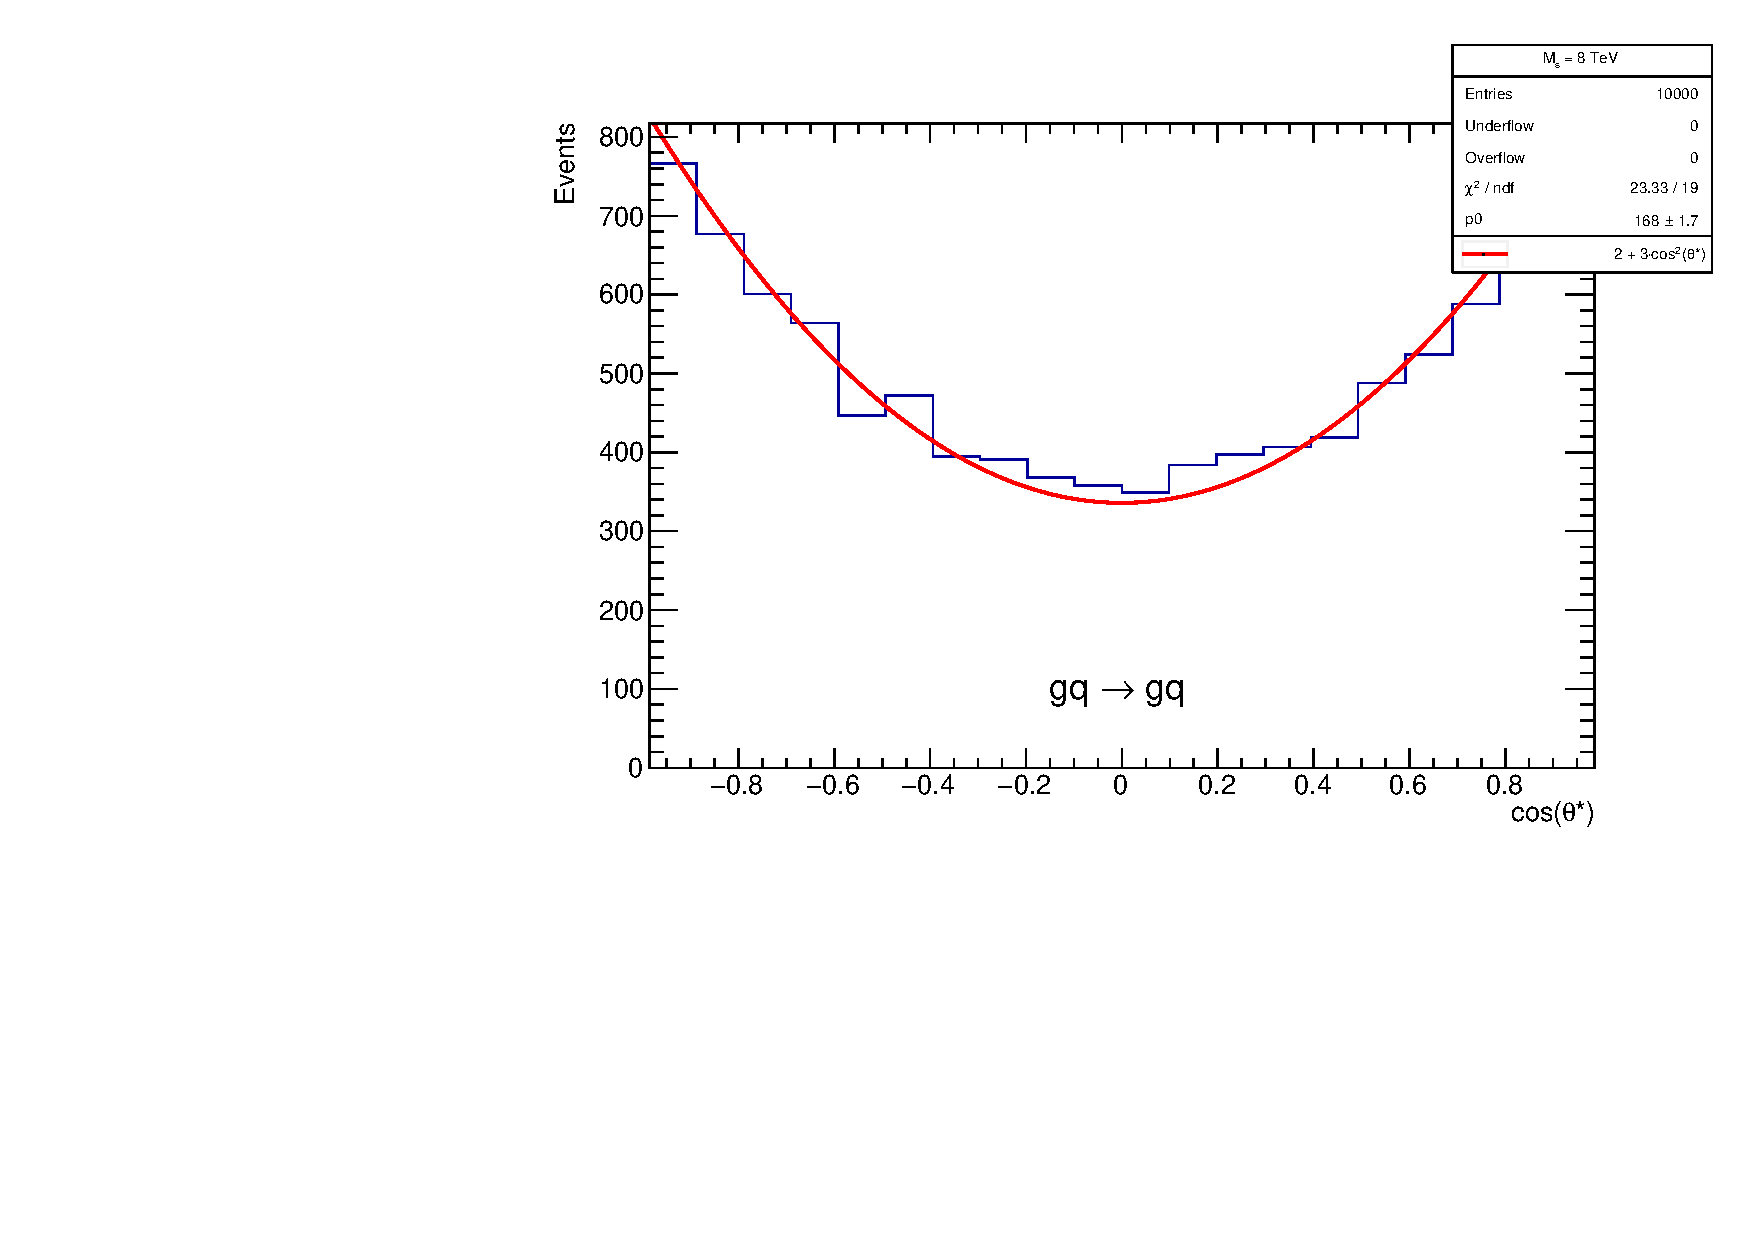
\includegraphics[width=0.45\linewidth]{../figures/strings/angle_gq_gq}
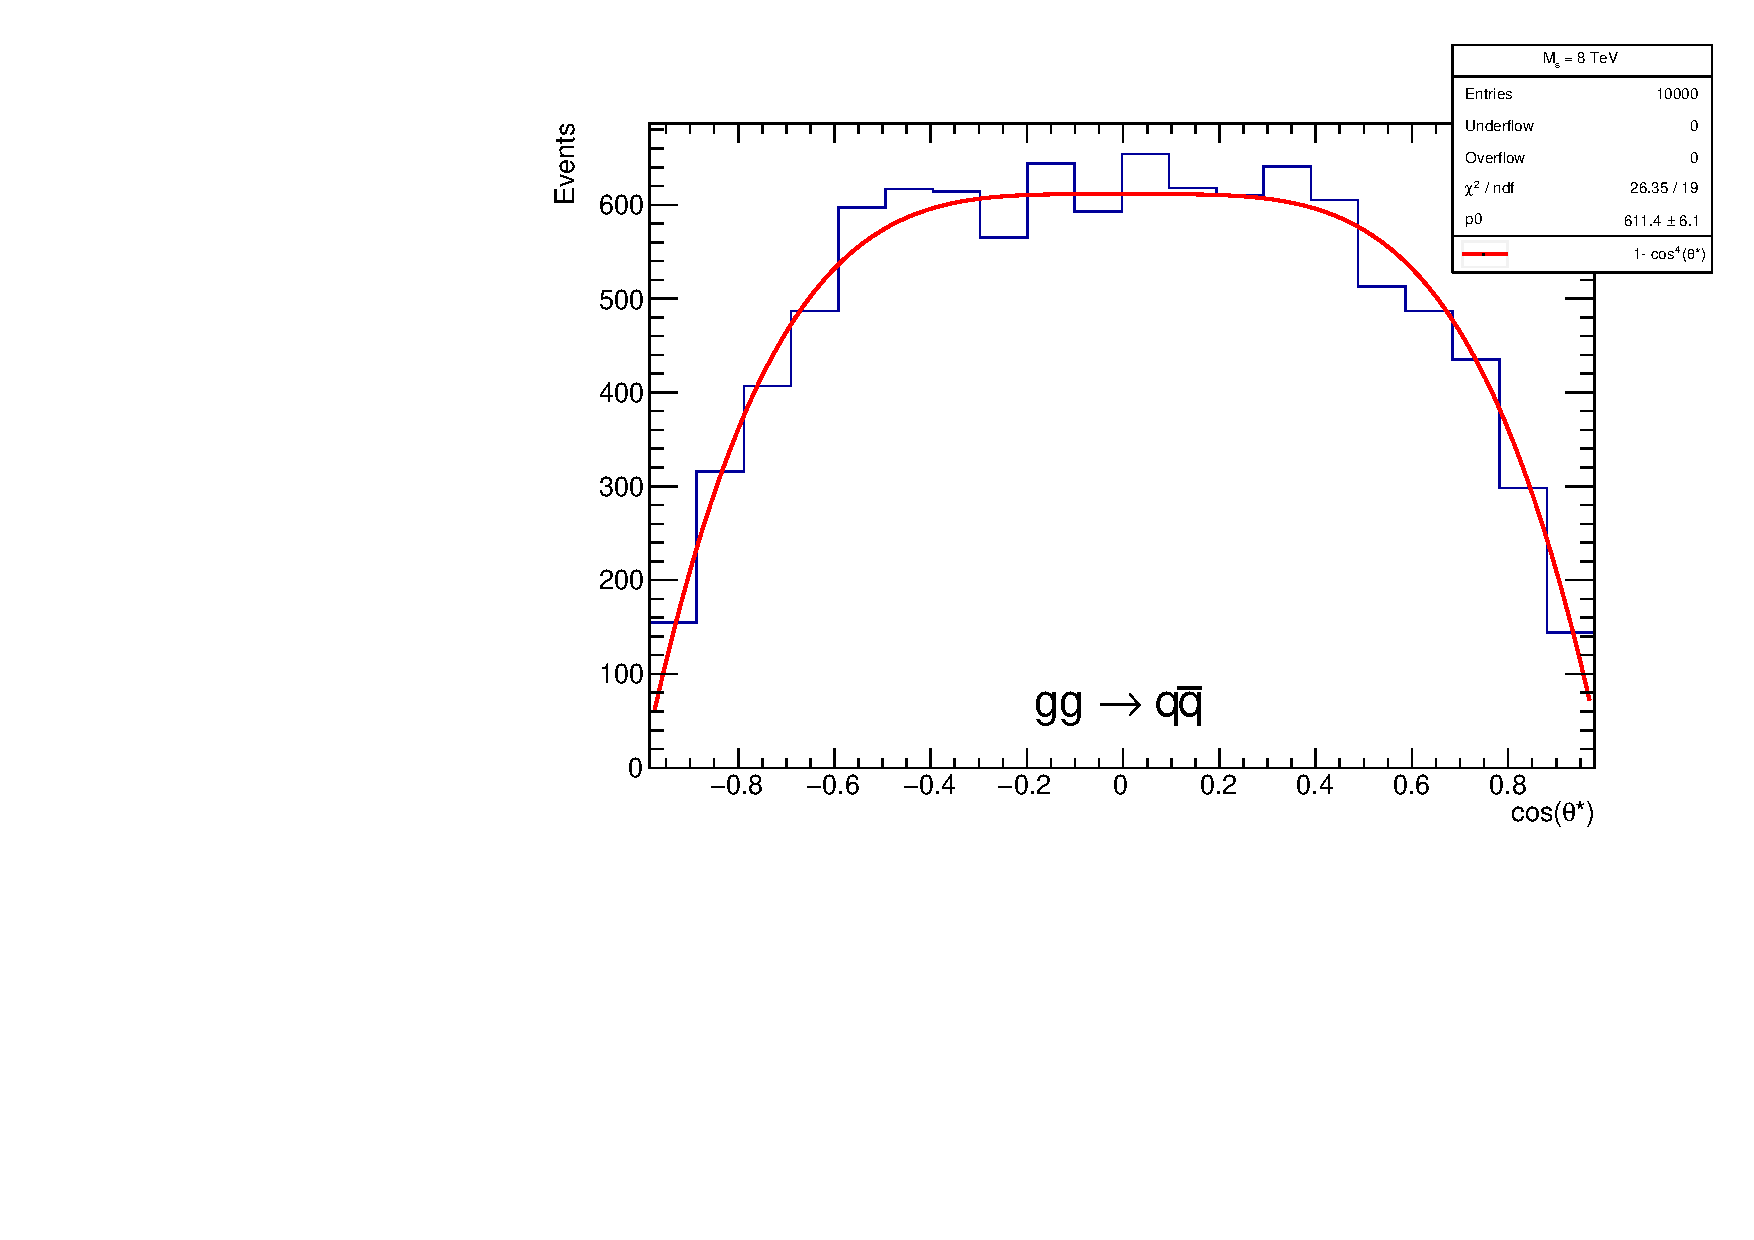
\includegraphics[width=0.45\linewidth]{../figures/strings/angle_gg_qq-bar}
\end{center}
\caption{Angular distribution of the outgoing partons from string
resonances in the centre of mass system:
(top-left) $gg\to gg$,
(top-right) $q\bar{q}\to gg$,
(bottom-left) $gq\to gq$,
(bottom-right) $gg\to q\bar{q}$.}
\label{fig:stringangle}
\end{figure}

The string resonance consist of a combination of excited quark, excited
gluon, and colour singlet states, depending on the subprocess.
In choosing the $y^*$ cut it is useful to examine the decay angular
distributions.
Figure~\ref{fig:stringangle} shows the angular distribution of the outgoing partons
in the centre of mass system for four different string resonance
subprocesses.
The case of string scale $\Ms = 8$~TeV is shown but the distributions
are similar for the other generated string scales.
The angular distribution for the process $g\bar{q}\to g\bar{q}$ (not
shown) is similar to $gq\to gq$.
The red curves show the calculated angular distributions for a string
mass equal to \Ms.

%%============================================

\subsection{\qstar signal samples}
\label{section:MCqStarSamples}

Table~\ref{tab:qStarSamps} shows the \qstar~samples used. Samples listed are the mc16a variant, the other samples use tags r10201 (mc16d) and r10724 (mc16e). The listed number of generated events is the total across all three MC campaigns.

\begin{table}[h]
        \centering
        \tiny
        \begin{tabular}{l|c|c|c}
                \hline\hline
                Dataset Container & Cross Section [fb] & N Gen Events \\
                \hline
                mc16\_13TeV.301299.Pythia8EvtGen\_A14NNPDF23LO\_ExcitedQ2000Lambda2000f1.deriv.DAOD\_EXOT2.e3855\_a875\_r9364\_p3654 & 2.3858e+04 & 40000 \\
                mc16\_13TeV.301300.Pythia8EvtGen\_A14NNPDF23LO\_ExcitedQ2500Lambda2500f1.deriv.DAOD\_EXOT2.e3855\_a875\_r9364\_p3654 & 6.2668e+03 & 40000 \\
                mc16\_13TeV.301301.Pythia8EvtGen\_A14NNPDF23LO\_ExcitedQ3000Lambda3000f1.deriv.DAOD\_EXOT2.e3855\_a875\_r9364\_p3654 & 1.8255e+03 & 40000 \\
                mc16\_13TeV.301302.Pythia8EvtGen\_A14NNPDF23LO\_ExcitedQ3500Lambda3500f1.deriv.DAOD\_EXOT2.e3855\_a875\_r9364\_p3654 & 5.8315e+02 & 40000 \\
                mc16\_13TeV.301303.Pythia8EvtGen\_A14NNPDF23LO\_ExcitedQ4000Lambda4000f1.deriv.DAOD\_EXOT2.e3840\_a875\_r9364\_p3654 & 1.9403e+02 & 40000 \\
                mc16\_13TeV.301304.Pythia8EvtGen\_A14NNPDF23LO\_ExcitedQ4500Lambda4500f1.deriv.DAOD\_EXOT2.e3855\_a875\_r9364\_p3654 & 6.5838e+01 & 40000 \\
                mc16\_13TeV.301305.Pythia8EvtGen\_A14NNPDF23LO\_ExcitedQ5000Lambda5000f1.deriv.DAOD\_EXOT2.e3855\_a875\_r9364\_p3654 & 2.2763e+01 & 40000 \\
                mc16\_13TeV.301306.Pythia8EvtGen\_A14NNPDF23LO\_ExcitedQ5500Lambda5500f1.deriv.DAOD\_EXOT2.e3855\_a875\_r9364\_p3654 & 7.8313e+00 & 40000 \\
                mc16\_13TeV.301307.Pythia8EvtGen\_A14NNPDF23LO\_ExcitedQ6000Lambda6000f1.deriv.DAOD\_EXOT2.e3840\_a875\_r9364\_p3654 & 2.7040e+00 & 40000 \\
                mc16\_13TeV.301308.Pythia8EvtGen\_A14NNPDF23LO\_ExcitedQ6500Lambda6500f1.deriv.DAOD\_EXOT2.e3855\_a875\_r9364\_p3654 & 9.3650e-01 & 40000 \\
                mc16\_13TeV.301309.Pythia8EvtGen\_A14NNPDF23LO\_ExcitedQ7000Lambda7000f1.deriv.DAOD\_EXOT2.e3855\_a875\_r9364\_p3654 & 3.3280e-01 & 40000 \\
                \hline\hline
        \end{tabular}
        \caption{\qstar~samples. %reconstructed with 50 ns settings
                \label{tab:qStarSamps}}
\end{table}

%%==========================================

\subsection{QBH signal samples}
\label{section:MCQBHgSamples}

Table~\ref{tab:qbhSamps} shows the QBH samples used. Samples listed are the mc16a variant, the other samples use tags r10201 (mc16d) and r10724 (mc16e). The listed number of generated events is the total across all three MC campaigns.

\begin{table}[h]
	\centering
	\tiny
	\begin{tabular}{l|c|c|c}
		\hline\hline
		Dataset Container & Cross Section (fb) & N Gen Events \\
		\hline
		mc16\_13TeV.303468.BlackMaxPythia8EvtGen\_A14CTEQ6L1\_LM1\_n6\_MthMD4000.deriv.DAOD\_EXOT2.e4184\_a875\_r9364\_p3654 & 1.7898e+04 & 40000 \\
		mc16\_13TeV.303469.BlackMaxPythia8EvtGen\_A14CTEQ6L1\_LM1\_n6\_MthMD5000.deriv.DAOD\_EXOT2.e4184\_a875\_r9364\_p3654 & 2.3475e+03 & 40000 \\
		mc16\_13TeV.303470.BlackMaxPythia8EvtGen\_A14CTEQ6L1\_LM1\_n6\_MthMD5500.deriv.DAOD\_EXOT2.e4184\_a875\_r9364\_p3654 & 8.4588e+02 & 40000 \\
		mc16\_13TeV.303471.BlackMaxPythia8EvtGen\_A14CTEQ6L1\_LM1\_n6\_MthMD6000.deriv.DAOD\_EXOT2.e4184\_a875\_r9364\_p3654 & 2.9958e+02 & 40000 \\
		mc16\_13TeV.303472.BlackMaxPythia8EvtGen\_A14CTEQ6L1\_LM1\_n6\_MthMD6500.deriv.DAOD\_EXOT2.e4184\_a875\_r9364\_p3654 & 1.0183e+02 & 40000 \\
		mc16\_13TeV.303473.BlackMaxPythia8EvtGen\_A14CTEQ6L1\_LM1\_n6\_MthMD7000.deriv.DAOD\_EXOT2.e4184\_a875\_r9364\_p3654 & 3.3335e+01 & 40000 \\
		mc16\_13TeV.303475.BlackMaxPythia8EvtGen\_A14CTEQ6L1\_LM1\_n6\_MthMD8000.deriv.DAOD\_EXOT2.e4184\_a875\_r9364\_p3654 & 2.9853e+00 & 40000 \\
		mc16\_13TeV.303476.BlackMaxPythia8EvtGen\_A14CTEQ6L1\_LM1\_n6\_MthMD8500.deriv.DAOD\_EXOT2.e4197\_a875\_r9364\_p3654 & 7.7647e-01 & 40000 \\
		mc16\_13TeV.303477.BlackMaxPythia8EvtGen\_A14CTEQ6L1\_LM1\_n6\_MthMD9000.deriv.DAOD\_EXOT2.e4197\_a875\_r9364\_p3654 & 1.8250e-01 & 40000 \\
		mc16\_13TeV.303478.BlackMaxPythia8EvtGen\_A14CTEQ6L1\_LM1\_n6\_MthMD9500.deriv.DAOD\_EXOT2.e4197\_a875\_r9364\_p3654 & 3.6260e-02 & 40000 \\
		mc16\_13TeV.303479.BlackMaxPythia8EvtGen\_A14CTEQ6L1\_LM1\_n6\_MthMD10000.deriv.DAOD\_EXOT2.e4197\_a875\_r9364\_p3654 & 6.0135e-03 & 40000 \\
		\hline\hline
	\end{tabular}
	\caption{QBH samples generated with the BlackMax generator.
		\label{tab:qbhSamps}}
\end{table}


%%==========================================

\subsection{MadGraph+Pythia8+EvtGen Z' samples}
\label{subsec:MCZprimeSamples}

For the significance studies of QQ selection, we consider the pure axial-vector
leptophobic \Zprime model described by the ATLAS-CMS Dark Matter Forum
Report \cite{Abercrombie:2015wmb}, in the specific scenario outlined in Ref.\cite{Chala:2015ama},
where dijet searches complement mono-jet-like searches in regions of
parameter space where the decay of the \Zprime to invisible particles is
kinetically suppressed.
%
In this model, the \Zprime arises from a simple extension of the Standard
Model (SM) with an additional $U(1)$ gauge symmetry and a Dirac
fermion Dark Matter particle that has charges only under this new
group. Assuming that some SM particles are also charged under this
group, the \Zprime can mediate interactions between the SM and DM. The DM
particle $\chi$ has a mass $m_{DM}$. The spin-1 \Zprime has mass \mMed.

The Dark Matter Forum reports models with vector or axial-vector couplings
between the spin-1 mediator $\Zprime$ and SM and DM fields, with the corresponding interaction Lagrangians:

\begin{align}
	\mathcal{L}_{\mathrm{vector}} &= \gq \sum_{q={u,d,s,c,b,t}}  \Zprime_{\mu} \bar{q}\gamma^{\mu}q + \gDM \Zprime_{\mu} \bar{\chiDM}\gamma^{\mu}\chiDM \\
	\mathcal{L}_{\mathrm{axial-vector}} &= \gq \sum_{q={u,d,s,c,b,t}}  \Zprime_{\mu} \bar{q}\gamma^{\mu}\gamma^5q + \gDM \Zprime_{\mu} \bar{\chiDM}\gamma^{\mu}\gamma^5\chiDM.
\end{align}

The parameters in the model are thus
\begin{equation}
\left\{~\gq,
~ \gDM,
~\mDM,
~\mMed,
\right\} \,.
\end{equation}

where ~\gq is the coupling of the \Zprime mediator to quarks, ~ \gDM
is its coupling to the Dark Matter fermion, ~\mDM is the mass
of the Dark Matter fermion and~\mMed is the \Zprime mass.

The two most relevant parameters of this model in the dijet search are the coupling of the \Zprime to quarks
as it drives the intrinsic width of the resonance, and the \Zprime mass. The Dark Matter mass is fixed at 10 TeV and the coupling to DM to 1.5, with
a negligible effect on the resonance width.
%
The values of \gq and \mMed have been kept consistent with the previous published dijet result.
The requested $\mMed$ points go up to 7~TeV and a \gq of 0.5 is used. The \gq of 0.5 corresponds to a width of 12\% of resonance mass. 
This is nearly the maximum width
that this search is sensitive to, without incurring in significant background distortion.

Table~\ref{tab:zpSamps} shows the Z' samples used for the significance studies of QQ selection. Samples listed are the mc16a variant, the other samples use tags r10201 (mc16d) and r10724 (mc16e). The listed number of generated events is the total across all three MC campaigns.

\begin{table}[h]
	\centering
	\tiny
	\begin{tabular}{l|c|c|c}
		\hline\hline
		Dataset Container & Cross section (fb) & N Gen Events \\
		\hline
		mc16\_13TeV.307794.MGPy8EG\_N30LO\_A14N23LO\_DMsA\_dijet\_mR1p5\_gSM0p05.deriv.DAOD\_EXOT2.e5687\_a875\_r9364\_p3654 & 1.1604E+02 & 40000\\
		mc16\_13TeV.307798.MGPy8EG\_N30LO\_A14N23LO\_DMsA\_dijet\_mR1p5\_gSM0p1.deriv.DAOD\_EXOT2.e5687\_a875\_r9364\_p3654 & 4.6565E+02 & 40000\\
		mc16\_13TeV.307799.MGPy8EG\_N30LO\_A14N23LO\_DMsA\_dijet\_mR2p0\_gSM0p1.deriv.DAOD\_EXOT2.e5687\_a875\_r9364\_p3654 & 1.1181E+02 & 40000\\
		mc16\_13TeV.307800.MGPy8EG\_N30LO\_A14N23LO\_DMsA\_dijet\_mR2p5\_gSM0p1.deriv.DAOD\_EXOT2.e5687\_a875\_r9364\_p3654 & 3.2083E+01 & 40000\\
		mc16\_13TeV.307801.MGPy8EG\_N30LO\_A14N23LO\_DMsA\_dijet\_mR1p5\_gSM0p15.deriv.DAOD\_EXOT2.e5687\_a875\_r9364\_p3654 & 1.0540E+03 & 40000\\
		mc16\_13TeV.307802.MGPy8EG\_N30LO\_A14N23LO\_DMsA\_dijet\_mR2p0\_gSM0p15.deriv.DAOD\_EXOT2.e5687\_a875\_r9364\_p3654 & 2.5414E+02 & 40000\\
		mc16\_13TeV.307803.MGPy8EG\_N30LO\_A14N23LO\_DMsA\_dijet\_mR2p5\_gSM0p15.deriv.DAOD\_EXOT2.e5687\_a875\_r9364\_p3654 & 7.3433E+01 & 40000\\
		mc16\_13TeV.307804.MGPy8EG\_N30LO\_A14N23LO\_DMsA\_dijet\_mR3p0\_gSM0p15.deriv.DAOD\_EXOT2.e5687\_a875\_r9364\_p3654 & 2.3616E+01 & 40000\\
		mc16\_13TeV.307805.MGPy8EG\_N30LO\_A14N23LO\_DMsA\_dijet\_mR3p5\_gSM0p15.deriv.DAOD\_EXOT2.e5687\_a875\_r9364\_p3654 & 8.2250E+00 & 40000\\
		mc16\_13TeV.307806.MGPy8EG\_N30LO\_A14N23LO\_DMsA\_dijet\_mR4p0\_gSM0p15.deriv.DAOD\_EXOT2.e5687\_a875\_r9364\_p3654 & 3.0540E+00 & 40000\\
		mc16\_13TeV.307807.MGPy8EG\_N30LO\_A14N23LO\_DMsA\_dijet\_mR1p5\_gSM0p2.deriv.DAOD\_EXOT2.e5687\_a875\_r9364\_p3654 & 1.8990E+03 & 40000\\
		mc16\_13TeV.307808.MGPy8EG\_N30LO\_A14N23LO\_DMsA\_dijet\_mR2p0\_gSM0p2.deriv.DAOD\_EXOT2.e5687\_a875\_r9364\_p3654 & 4.5869E+02 & 40000\\
		mc16\_13TeV.307809.MGPy8EG\_N30LO\_A14N23LO\_DMsA\_dijet\_mR2p5\_gSM0p2.deriv.DAOD\_EXOT2.e5687\_a875\_r9364\_p3654 & 1.3406E+02 & 40000\\
		mc16\_13TeV.307810.MGPy8EG\_N30LO\_A14N23LO\_DMsA\_dijet\_mR3p0\_gSM0p2.deriv.DAOD\_EXOT2.e5687\_a875\_r9364\_p3654 & 4.3946E+01 & 40000\\
		mc16\_13TeV.307811.MGPy8EG\_N30LO\_A14N23LO\_DMsA\_dijet\_mR3p5\_gSM0p2.deriv.DAOD\_EXOT2.e5687\_a875\_r9364\_p3654 & 1.5686E+01 & 40000\\
		mc16\_13TeV.307812.MGPy8EG\_N30LO\_A14N23LO\_DMsA\_dijet\_mR4p0\_gSM0p2.deriv.DAOD\_EXOT2.e5687\_a875\_r9364\_p3654 & 6.0510E+00 & 40000\\
		mc16\_13TeV.307813.MGPy8EG\_N30LO\_A14N23LO\_DMsA\_dijet\_mR5p0\_gSM0p2.deriv.DAOD\_EXOT2.e5687\_a875\_r9364\_p3654 & 1.1820E+00 & 40000\\
		mc16\_13TeV.307814.MGPy8EG\_N30LO\_A14N23LO\_DMsA\_dijet\_mR2p5\_gSM0p3.deriv.DAOD\_EXOT2.e5687\_a875\_r9364\_p3654 & 3.2383E+02 & 40000\\
		mc16\_13TeV.307815.MGPy8EG\_N30LO\_A14N23LO\_DMsA\_dijet\_mR3p0\_gSM0p3.deriv.DAOD\_EXOT2.e5687\_a875\_r9364\_p3654 & 1.1080E+02 & 40000\\
		mc16\_13TeV.307816.MGPy8EG\_N30LO\_A14N23LO\_DMsA\_dijet\_mR3p5\_gSM0p3.deriv.DAOD\_EXOT2.e5687\_a875\_r9364\_p3654 & 4.1961E+01 & 40000\\
		mc16\_13TeV.307817.MGPy8EG\_N30LO\_A14N23LO\_DMsA\_dijet\_mR4p0\_gSM0p3.deriv.DAOD\_EXOT2.e5687\_a875\_r9364\_p3654 & 1.7550E+01 & 40000\\
		mc16\_13TeV.307818.MGPy8EG\_N30LO\_A14N23LO\_DMsA\_dijet\_mR5p0\_gSM0p3.deriv.DAOD\_EXOT2.e5687\_a875\_r9364\_p3654 & 4.2110E+00 & 40000\\
		mc16\_13TeV.307819.MGPy8EG\_N30LO\_A14N23LO\_DMsA\_dijet\_mR6p0\_gSM0p3.deriv.DAOD\_EXOT2.e5687\_a875\_r9364\_p3654 & 1.5110E+00 & 40000\\
		mc16\_13TeV.307820.MGPy8EG\_N30LO\_A14N23LO\_DMsA\_dijet\_mR4p0\_gSM0p4.deriv.DAOD\_EXOT2.e5687\_a875\_r9364\_p3654 & 4.0692E+01 & 40000\\
		mc16\_13TeV.307821.MGPy8EG\_N30LO\_A14N23LO\_DMsA\_dijet\_mR5p0\_gSM0p4.deriv.DAOD\_EXOT2.e5687\_a875\_r9364\_p3654 & 1.1296E+01 & 40000\\
		mc16\_13TeV.307822.MGPy8EG\_N30LO\_A14N23LO\_DMsA\_dijet\_mR6p0\_gSM0p4.deriv.DAOD\_EXOT2.e5687\_a875\_r9364\_p3654 & 4.4510E+00 & 40000\\
		mc16\_13TeV.307823.MGPy8EG\_N30LO\_A14N23LO\_DMsA\_dijet\_mR7p0\_gSM0p4.deriv.DAOD\_EXOT2.e5687\_a875\_r9364\_p3654 & 2.1830E+00 & 40000\\
		mc16\_13TeV.307824.MGPy8EG\_N30LO\_A14N23LO\_DMsA\_dijet\_mR4p0\_gSM0p5.deriv.DAOD\_EXOT2.e5687\_a875\_r9364\_p3654 & 8.1795E+01 & 40000\\
		mc16\_13TeV.307825.MGPy8EG\_N30LO\_A14N23LO\_DMsA\_dijet\_mR5p0\_gSM0p5.deriv.DAOD\_EXOT2.e5687\_a875\_r9364\_p3654 & 2.5066E+01 & 40000\\
		mc16\_13TeV.307826.MGPy8EG\_N30LO\_A14N23LO\_DMsA\_dijet\_mR6p0\_gSM0p5.deriv.DAOD\_EXOT2.e5687\_a875\_r9364\_p3654 & 1.0406E+01 & 40000\\
		mc16\_13TeV.307827.MGPy8EG\_N30LO\_A14N23LO\_DMsA\_dijet\_mR7p0\_gSM0p5.deriv.DAOD\_EXOT2.e5687\_a875\_r9364\_p3654 & 5.2180E+00 & 40000\\
		\hline\hline
	\end{tabular}
	\caption{MadGraph+Pythia8+EvtGen Z' samples used for the significance studies of QQ selection.
		\label{tab:zpSamps}}
\end{table}

%==================================

%%%%%%%%%%%%%%%%%%%%%%%%%%%%%%%%%%%%%%%%%%%%%%%%%%%%%%%%%%%%%%%%%%%%%%%%%%%%%%%%
